\chapter*{Introduction}
The handshake event, commonly used, is a natural human interaction and is extensively used worldwide in events like: greetings, introduction routine between human beings and agreements. 
The scientific approach to handshake between a human and a robot, therefore, must intrinsically deal with low levels of human interaction and some assumption must be done in order to focus on the task.
The handshake event can be divided in two steps: the approaching and handshaking. This work is focused on the haptic sense involved during the handshake, knowing that the approaching is mainly executed using non haptic senses(f.i. vision).\\ The consensus is a parameter that allow the human to evaluate a handshake mixing aspects like: duration of the event, dynamics, force exchanged.
An important part of this work is to test different controllers with the purpose of evaluating the consensus using closed loop controllers. 
  
%Many research teams all over the world are focused on the human-robot physical interaction, this opens the topic to an interesting scientific discussion.  


\chapter{The state of the Art}
Develop a robot capable of performing a smooth human-like handshake is still a highly interested topic in the scientific literature.
A natural handshake between two humans is a very complex task to replicate, this work just focuses on the interaction force between the artificial hand and the human hand.
The consensus is a complex task to encode inside a robot, the human will easily distinguish the event with respect to another human or to a robot. A human will take into consideration the skin feedbacks like: the temperature, the humidity and the softness. These are some characteristics that are still not embedded into the hardware available in the market. The aspect taken in consideration in this work is the grasping force exchanged in the handshake. 
Robots, nowadays, are highly involved in industries where mostly they have to execute repetitive tasks. These kind of robots, when deals in grasping objects, commonly uses multi purposes grippers \cite{multipurposegripper}, therefore, an accurate choice has been done on the hardware to use in this work. 
%The grasping force exchanged in the human-robot handshake event is a complex value to identify, this work is estimating the grasping force from values which can be clearly identified. 


\cite{facialexpressions}
\cite{mirrorgame}
\cite{papageorgiou}

\section{The Idea}
The idea is to create a closed loop controller for the human-robot handshake event, using Pisa/IIT SoftHand produced for research purposes at Universit\`a degli studi di Pisa and Istituto Italiano di Tecnologia (IIT) and upgrading it with four independent FSR sensors which uses an Arduino uno in order to communicate the data.
The FSR sensors are located on the robotic hand so there are no wearing device on the human hand during the execution of the experiments.
This choice leads the work to be focused on the theoretical part of the handshake event, and potentially reach robust results. We are focusing on a general human-robot handshake, knowing that the interaction can vary with participants, f.i. the participant's hand size is affecting the firsts contact points or nominal strength to apply in the handshake can be affected by prior expectations. It is more meaningful then, to study individual differences once the generic case has been studied.
The chosen robotic hand (Pisa/IIT SoftHand) has 19 degrees of freedom and its main characteristic a single dc motor that is pulling a tendon which is embedded in each finger. This physical approach results in an under actuated robotic hand which can be controlled only by the dc motor and can easily adapt to different configurations without modifying the reference position. 

\chapter{Hardware setup}
The hardware must be physically merged in order to reach the goal of a closed loop controller for a handshake. From early approaches as \cite{espen}, an estimation of the human palm has been used.  The \textit{sensorized palm} idea was to approximate the human palm which is the part of the hand mostly interested during a handshake.
The figure \ref{fig:sensorsONhand} shows the position in which the sensors are placed, in particular the n. 1, 2, 3 are placed according studies in \cite{espen}, the sensor n. 4 is placed in order to help the human-thumb force applied during the grasp.\\ \\

\begin{figure}[h]
  \centering
  \begin{minipage}[b]{0.4\textwidth}
    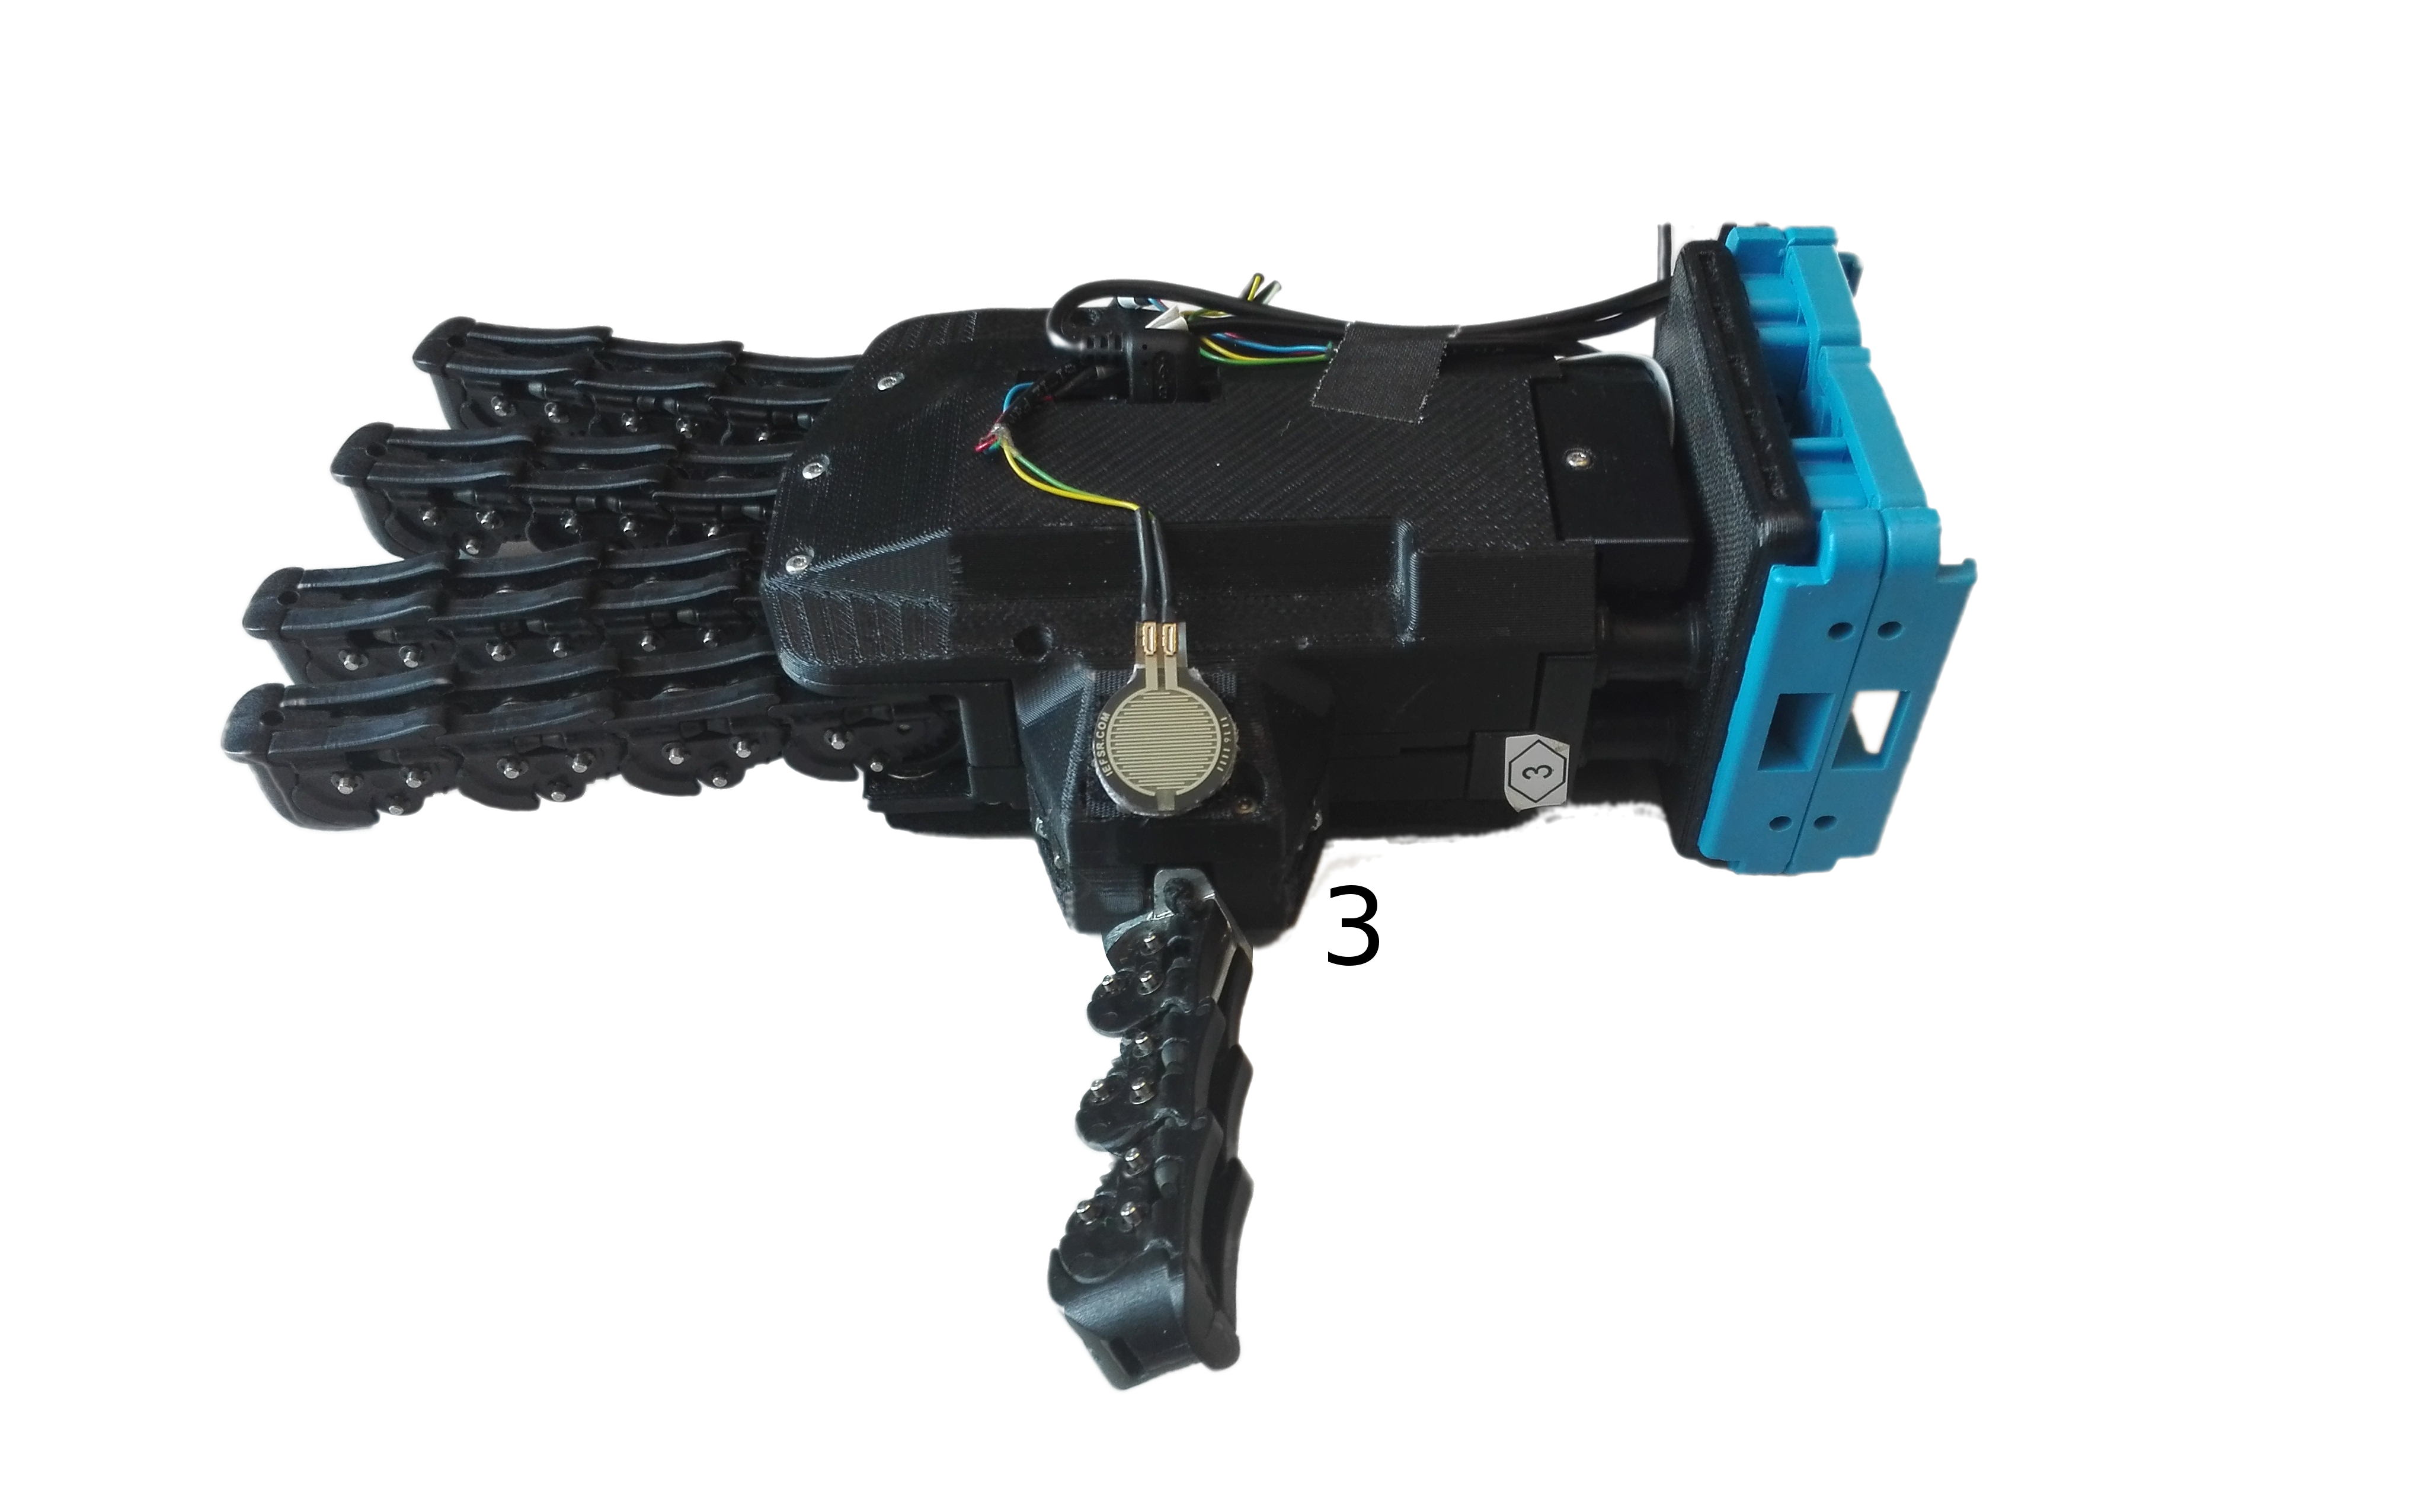
\includegraphics[width=\textwidth]{Figure/qbhand1.png}
    
  \end{minipage}
  \hfill
  \begin{minipage}[b]{0.4\textwidth}
    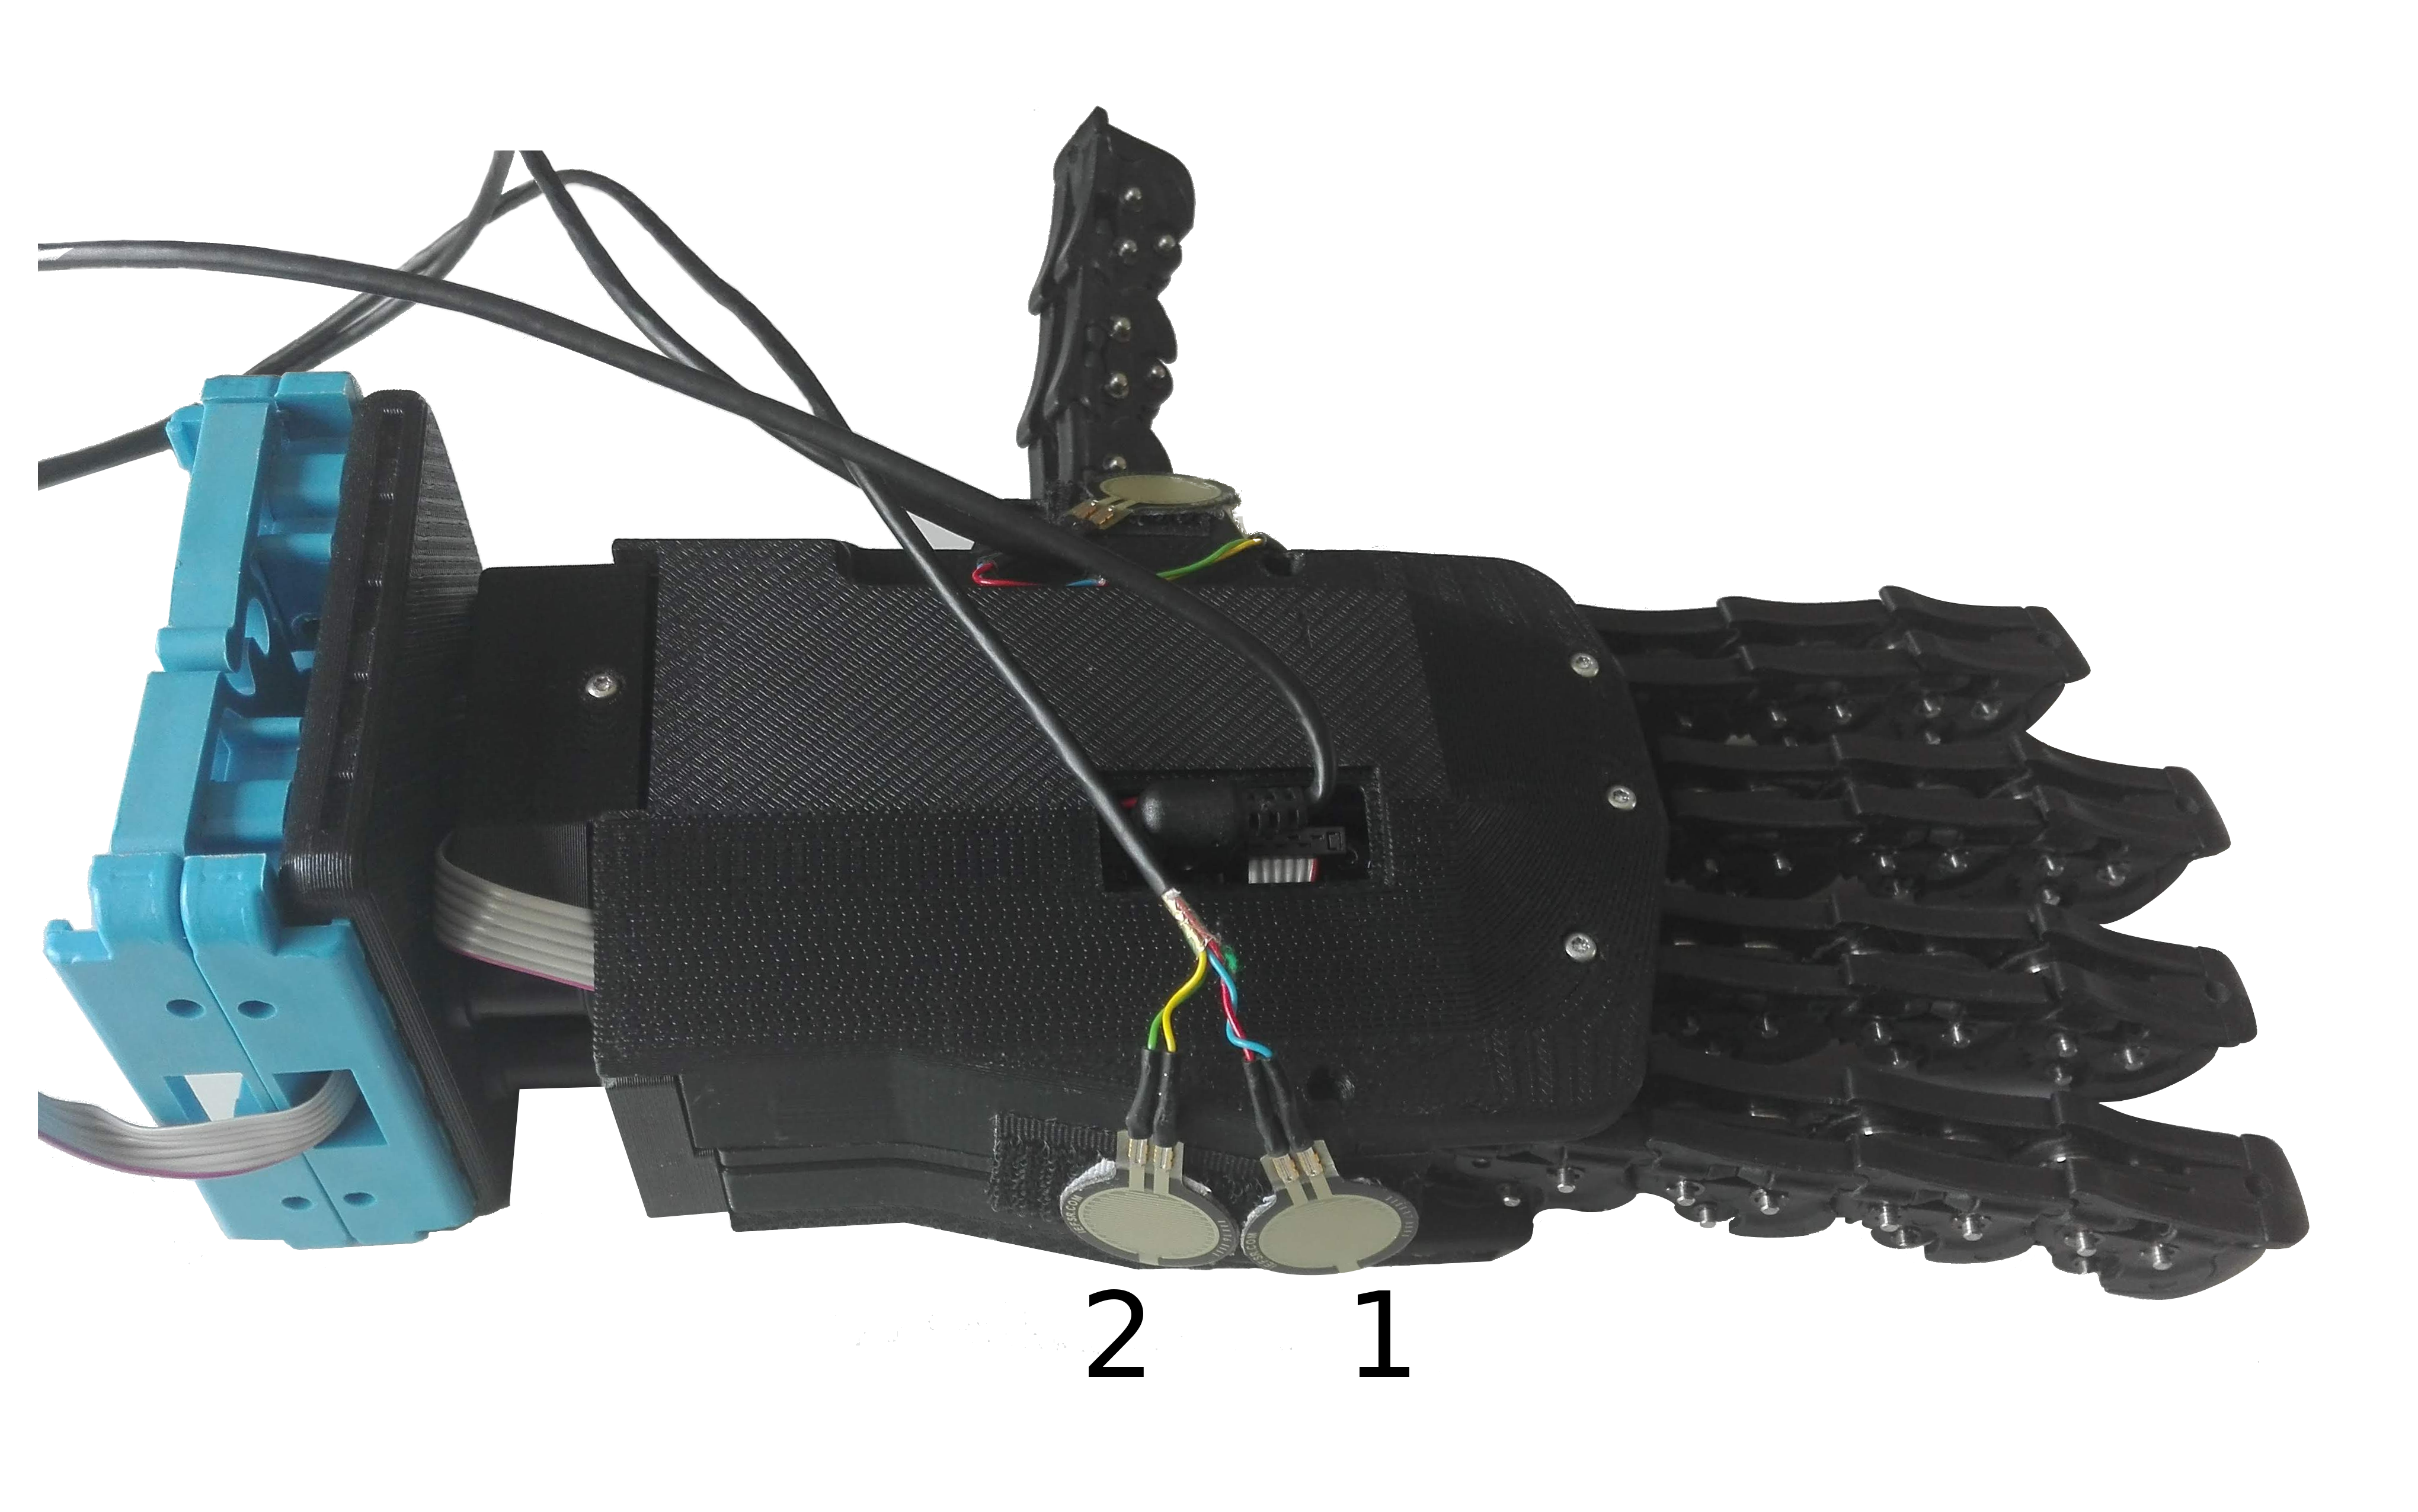
\includegraphics[width=\textwidth]{Figure/qbhand2.png}
  \end{minipage}
  \label{fig:sensorsONhand}
  \caption{Pisa/IIT SoftHand with FSR sensors for handshake}
\end{figure}

\section{The Pisa/IIT SoftHand}
The Pisa/IIT SoftHand is a simple, robust and effective hand designed for grasping and soft manipulation presented in \cite{catalanopisa}, the hardware is provided with a controller developed by the same group which implements a proportional controller [fig. \ref{Fig:Pr}] on the motor position. This enables the researchers to control the Pisa/IIT SoftHand with a reference position, without dealing with the current control of the motor.\\
\begin{figure}[h]
\centering
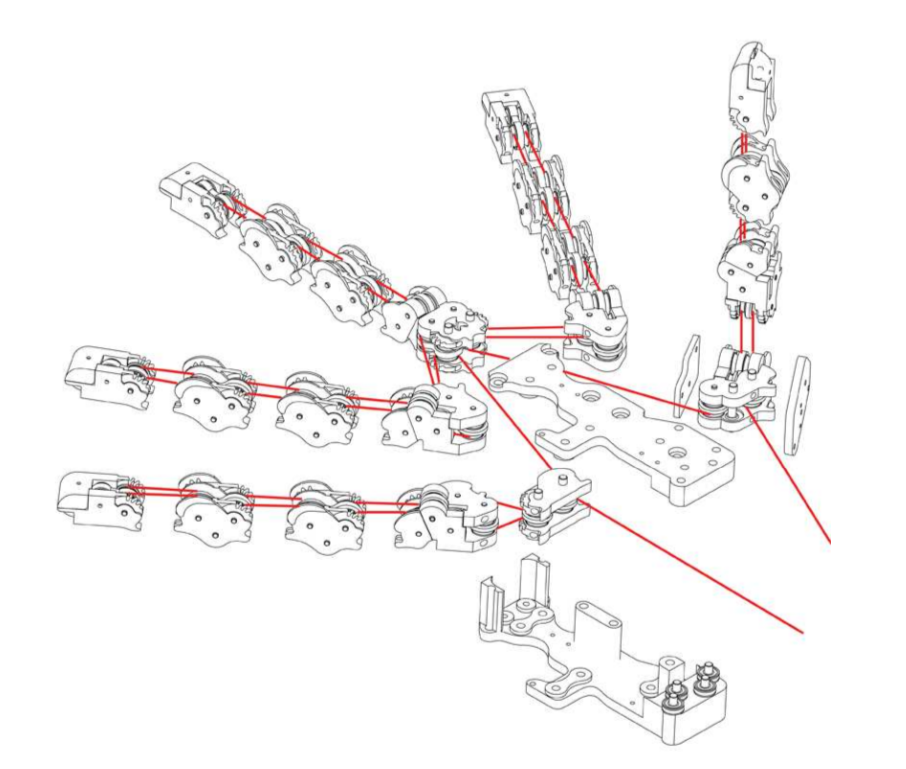
\includegraphics[width=0.6\textwidth]{Figure/softhand.png}
\caption{Exploited view of the modules of Pisa/IIT SoftHand}
\label{Fig:Softhand}
\end{figure}\\
The proportional coefficient can be set up as preferred since its encode in ROS as a \textit{rosparam}, this parameter is thought to range between 0 and 1.0. Setting the parameter to 1.0 is minimizing the error value $e(t)$  between the setpoint $r(t)$ and the output $y(t)$.

The successful idea in the design of Pisa/IIT SoftHand can be found in the flexibility of the joints and the wide range of usage.

The reference position $r(t)$ has no 1:1 correspondence with the single physical position of each finger. Having a single motor to control makes the robotic hand really easy to control but introduce uncertainty on the position of each finger. A tendon is running through all the fingers and is pulled by the internal dc motor, therefore, the only available information is the overall tick-position of the Pisa/IIT SoftHand. The controller used $C(s)$ is a simple constant controller with value ranges from 0 to 1. 

\begin{figure}[h]
\centering
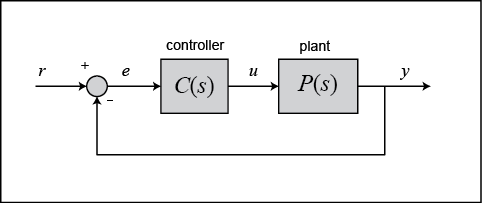
\includegraphics[width=0.3\textwidth]{Figure/feedbackP.png}
\caption{Block Diagram Proportional controller in a feedback loop}
\label{Fig:Pr}
\end{figure}


\section{The Sensors}
The core of the closed loop control is to have a feedback in the whole system which is proportional to the force applied during the handshake from the human. 
\begin{wrapfigure}{R}{0.3\textwidth}
\centering
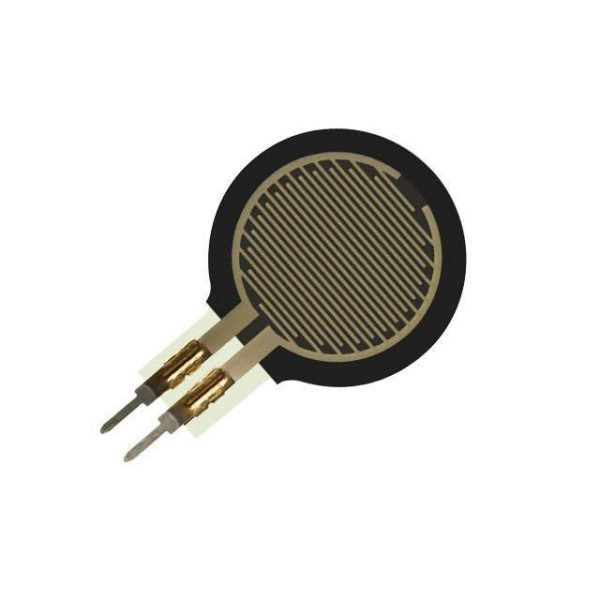
\includegraphics[width=0.25\textwidth]{Figure/fsrsingle1.jpg}
\caption{FSR 13mm}
\label{Fig:FSRsingle}
\end{wrapfigure}

The sensors used in this work are Force Sensitive Resistors Fig. \ref{Fig:FSRsingle} measuring the force applied from the human to the Pisa/IIT SoftHand, in order to decouple this force from the one applied from the Pisa/IIT SoftHand to the human hand, \cite{espen} has been used and the physical interaction during the handshake has been setted up accordingly.
FSR sensors are devices that allow to measure static and/or dynamic forces applied on the sensing area, through the variation of its electric resistance. The main advantage of these devices is the low cost per-unit, little space required for installation (thickness under 1.25mm) and the force sensitivity range up to 20N.\\


As robust polymer thick film devices, the FSRs, exhibit a decrease in resistance with increase in force applied to the surface. By theory is considered that when a force is applied the resistance changes approximately linear in a logarithmic plot \cite{fsrdatasheet}.
A simple force to voltage conversion is physically implemented as suggested the manifacturer, in fig. \ref{Fig:FSRcircuit} is shown a snippet of the above mentioned data sheet. For this work \textit{RM} is fixed to $3.3 k \Omega $. 
\begin{figure}[ht]
\centering
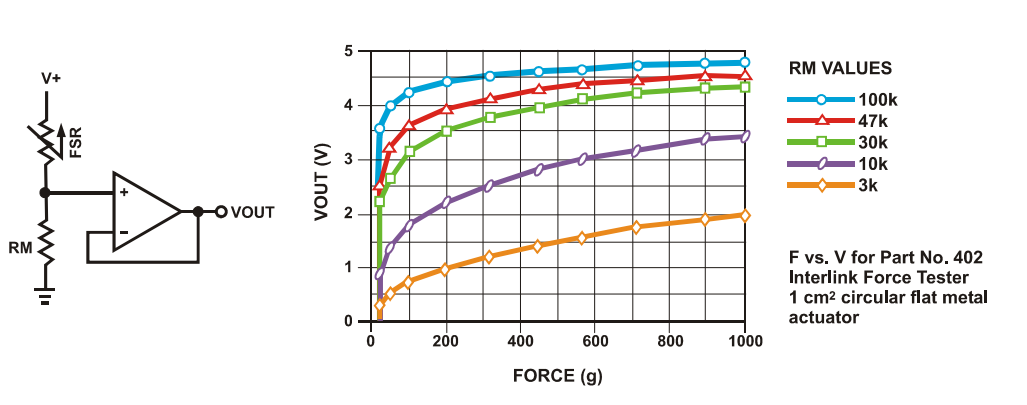
\includegraphics[width=0.6\textwidth]{Figure/fsr.png}
\caption{FSR Datasheet snippet}
\label{Fig:FSRcircuit}
\end{figure}
These mentioned sensors are the more natural choice for handshake experiments since their thickness keeps the size of the Pisa/IIT SoftHand reasonable for human-robot handshake. The number of FSR sensors involved in the calibration experiment is two, instead the amount of FSR sensors chosen for the human-robot handshake is four. Ideally using more sensors allow to get more relevant data but the surface available on the Pisa/IIT SoftHand is limited. The choice in the number of FSR sensors comes from the trade off between using lots of FSR sensors but with a smaller area and using a smaller amount of sensors but with higher area. The first configuration does not ensure the contact among experiments with different participants and the second configuration leads to physical bending of the sensors and influence the consistency of the readings. %A calibration method must be used in order to have robust results.

\subsection{Calibration of FSRs}
The calibration procedure of a sensor is a really important task, since it allow to compare experiments and to provide consistent results. 
The first voltage-to-force relation for the FSRs comes from a manufacturer sketch which is returning force with measures standard of grams.
As shown in \cite{calibFSR}, load cells can be used as 'ground truth' to calibrate force sensitive resistors to provide informations in Newtons. 
Using a \textit{sensorized palm} developed in \cite{espen}, sketched in Fig. \ref{fig:dummi} which embeds a load cell and placing the FSR sensors accordingly to the main direction of the force on this \textit{sensorized palm}; values from FSRs and the load cell are compared.
Mathematical regression tools have been used in order to find a model that explain the values from the sensors compared to the force of the load cell.
Although an exact calibration of FSR sensors is not the target of this work, a first order model has been fitted to the data in the force-range of interest of this work.
The configuration for the calibration experiment, with the \textit{sensorized palm} and two FRS sensors placed on top is shown in Fig. \ref{fig:dummifsr}. In order not to add complexity to this task, is assumed that using two FSR are sufficient to fit a model to the FSR sensors involved in the handshake.

\begin{figure}[h]
  \centering
  \begin{minipage}[b]{0.4\textwidth}
    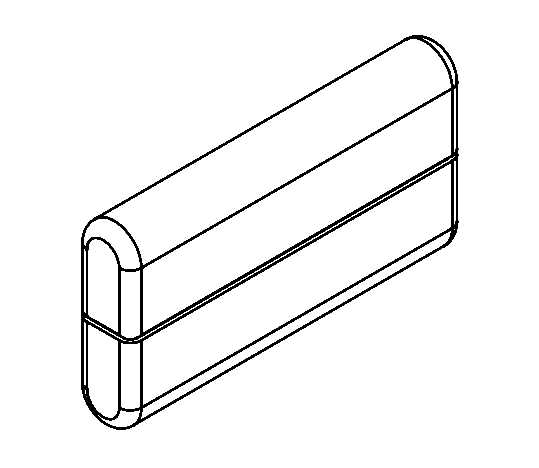
\includegraphics[width=\textwidth]{Figure/dummipalm.png}
    \caption{Sensorized palm}
  \label{fig:dummi}
  \end{minipage}
  \hfill
  \begin{minipage}[b]{0.4\textwidth}
    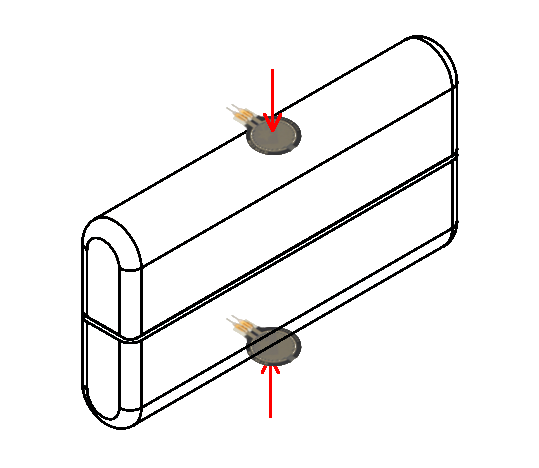
\includegraphics[width=\textwidth]{Figure/dummipalmfsr.png}
    \caption{Sensorized palm with FSR sensors}
    \label{fig:dummifsr}
  \end{minipage}
  %\caption{FSR sensors position on sensorized palm}
\end{figure}

 



\chapter{Software setup}
The experiments described needs a software capable of exchanging informations between robots, without the interaction of a human, therefore the Robot Operative System has been chosen in order to manage the informations between the devices involved in these experiments.  
\section{Ros}
The Robot Operative System (ROS) is a set of frameworks and libraries useful for robot software development. The logic of this software is really intuitive, it lets the developers to represent a device as node inside a graph. Each device is therefore a node inside this graph, and all the communications are going through a main node, also called master node, which takes care about forwarding the informations between nodes.
\section{Nodes}
\subsection{Pisa\textbackslash IIT SoftHand node}
\subsection{FSRs node}
\subsection{Auxiliary nodes}

\chapter{Open Loop Experiments}
\section{Step input}
\section{Pseudorandom input}

\chapter{Closed Loop controllers}
\chapter{Results}

\chapter*{Conclusion}
This project applies learning \cite{art:rif.1} techniques to MNIST handwritten dataset. As we can see in the previous confusion matrix the accuracy of the final work is $97.6\%$. The overall idea is to train \emph{autoenc1},  \emph{autoenc2} and \emph{softmax1} once per time and to crop the nets in order to have coherents dimension between network interconnections. At the end of \cite{book:rif.2}this process we stack all the partial neural network together and the deep neural network come to life. \\The satisfaction behind this project can be experimented by running the file "MNIST\textunderscore drawsim.m" which is a matlab function that allows the user to draw a digit and returns the correct digit value 97,6 times over 100.